\documentclass[a4paper]{article} % {scrartcl} % for \subtitle
\usepackage[italian]{babel} 
\usepackage[utf8]{inputenc}
\usepackage[T1]{fontenc}
\usepackage{graphicx}
\usepackage{subfigure}
\usepackage{amsmath,amssymb, amsthm}
\usepackage{tabularx}
% Customized hyper references
\usepackage[pdftex,colorlinks]{hyperref}
%% Collegamenti ipertestuali in blu
%% in modo che siano visibili anche stampati
\hypersetup{%
            citecolor=blue,%
            filecolor=blue,%
            linkcolor=blue,%
            urlcolor=blue}

\author{Gianmarco Brocchi}
% \title{Weighted Nonnegative Matrix Factorization \\
% and Face Feature Extraction \\ - \\ un'implementazione}
\title{Face Feature Extraction: un'implementazione}
% \subtitle{Un'implementazione}
\date{\today}

\begin{document}
\maketitle

\section{Il problema}
Data un'immagine (o una raccolta di immagini), questa viene rappresentata come matrice numerica di un certo ordine. Si vuole approssimare tale matrice con il prodotto di due matrici di ordine inferiore mantenendo più dati possibili in specifiche zone della matrice di partenza.

\paragraph{Soluzione implementata}
Per ottenere il risultato cercato su matrici rappresentanti volti (vedi \ref{faces}), viene utilizzata la NMF\footnote{Nonnegative Matrix Factorization - Fattorizzazione Matriciale Non negativa}, dove la matrice di partenza $A$ di ordine $(n \times m)$ viene approssimata come prodotto delle matrici non negative $U$ e $V$ di ordine $(n \times k)$ e $(k \times m)$.

Al fine di preservare certe zone della matrice di partenza viene usata la WNMF\footnote{\emph{Weighted} Nonnegative Matrix Factorization - Fattorizzazione Matriciale \emph{Pesata} Non negativa} la quale sfrutta una matrice di pesi $W$ dello stesso ordine di $A$ per enfatizzare specifiche zone di dati durante l'approssimazione.

\section{Il software}
È stato sviluppato un software in \texttt{FORTRAN 90} che implementa la WNMF su una singola immagine o su una collezione di immagini in input.

Tale software può essere scaricato via \texttt{git} all'indirizzo:
\begin{center} \url{http://poisson.phc.unipi.it/~brocchi/git/WNMF/} \end{center}

Per la compilazione e l'esecuzione si veda le istruzioni \ref{makefile}.

\subsection{L'algoritmo}
Usando l'algoritmo suggerito in \ref{wnmf} e adattato come accennato in \ref{libnmf}, viene applicata la WNMF a una matrice in input $A$di ordine $(n \times m)$ nel seguente modo:
\begin{enumerate}
\item Viene generata la matrice dei pesi $W$ (vedi \ref{W});
\item Vengono generate in maniera casuale le matrici $U$ e $V$, di ordine $(n \times k)$ e $(k \times m)$, dato $k$;
  \item Vengono eseguiti iterativamente:
    \begin{itemize}
    \item[\textbf{a})] Viene calcolata $UV$ e vengono aggiornate le matrici $U$ e $V$ (vedi \ref{updaterules});
    \item[\textbf{b})] Viene calcolata la divergenza di Kullback-Leibler\footnote{diremo semplicemente \emph{divergenza KL} e la indicheremo con $D(A\lVert UV)$, (vedi \ref{KL-div})} tra la matrice di partenza $A$ e l'approssimazione $UV$ finora ottenuta;
    \end{itemize}
\end{enumerate}
Gli ultimi due punti vengono ripetuti fino a che non si raggiunge il numero massimo di iterazioni fissato o finché la divergenza di Kullback-Leibler non scende sotto una soglia fissata.

% da enfatizzare certe parti della matrice che le rappresenta. Useremo immagini di volti per evidenziare la parte centrale del viso.

\paragraph{Matrice dei pesi}\label{W}
La matrice dei pesi $W$ viene generata a partire dalle dimensioni dell'immagine in input, i suoi elementi sono dati da:

\[ W(i,j) = e^{-\frac{d}{\sigma^2}} \]

dove $d$ è la distanza del punto $(i,j)$ dal centro dell'immagine (ovvero $(56,5 ; 46,5)$ per una matrice $112 \times 92$); $\sigma$ è un parametro fissato a $30$.

\paragraph{Regole di aggiornamento}\label{updaterules}
Le matrici $U$ e $V$ vengono aggiornate nel modo seguente\footnote{Con $\circ$ si indica di \emph{prodotto di Hadamard}, mentre con $\frac{[X]}{[Y]}$ si indica la \emph{divisione di Hadamard}, entrambe effettuate componente a componente; con $\log_{\circ}$ si indica il logaritmo delle componenti.}:

\[ \frac{[V]}{[U^tW]} \circ \left( U^t \frac{[W \circ A]}{[UV]} \right) \rightarrow V \text{ , } \frac{[U]}{[WV^t]} \circ \left( \frac{[W \circ A]}{[UV]}V^t \right) \rightarrow U \]

\vspace{5mm}
In \ref{wnmf} viene mostrato come la divergenza KL pesata $D_W(A\lVert UV)$ non aumenti con questi aggiornamenti di $U$ e $V$, se queste sono non negative.

\paragraph{Divergenza di Kullback-Leibler}\label{KL-div}
La \emph{Kullback-Leibler Divergence} è una stima non simmetrica della differenza tra due distribuzioni di probabilità. Nello specifico, date due distribuzioni di probabilità $P$ e $Q$, la divergenza di Kullback–Leibler di $Q$ da $P$, indicata con $D_{KL}(P \lVert Q)$, è una misura dell'informazione persa quando $Q$ è usata per approssimare $P$. Tale misura è spesso usata nell'approssimazione di immagini, come nel nostro caso.

Data la matrice $A$, la sua ``distanza'' dalla fattorizzazione $UV$ è data da:
\[ D(A \lVert UV) := \sum_{ij} \left[ A \circ \log_{\circ} \frac{[A]}{[UV]} - A + UV \right]_{ij} \]

Data $A$, stimeremo la sua distanza dalla fattorizzazione $UV$ con la \emph{KL-divergence \emph{pesata} con $W$} nel seguente modo:
\[ D_W(A \lVert UV) := \sum_{ij} \left[ \textbf{W} \circ \left( A \circ \log_{\circ} \frac{[A]}{[UV]} - A + UV \right) \right]_{ij} \]

\paragraph{I dati}\label{faces}
L'algoritmo lavora su dati ottenuti dall'\texttt{ORL} face database [vedi \ref{ORL}].
Nello specifico si tratta di $400$ volti ($10$ immagini per $40$ soggetti). Le immagini sono in formato PGM\footnote{Portable Gray Map format}, ovvero in scala di grigi; tali immagini possono essere in formato RAW o ASCII, nel primo i valori di grigio sono memorizzati come semplici byte, nel secondo sono rappresentati da un intero compreso tra 0 e 255. \\ 
(Le immagini dell'\texttt{ORL} erano nel primo formato, è quindi necessario convertirle in ASCII: il software si occupa anche di questo [vedi \ref{paragr:conversione}]).

\subsection{Implementazione}
Di default il programma si occupa dell'approssimazione di più immagini simultaneamente.
È possibile cambiare questo comportamento compilando nel \texttt{Makefile} la subroutine \texttt{read.f90} al posto di \texttt{wnmf.f90} (vedi \ref{makefile}).

\paragraph{Conversione}\label{paragr:conversione}
Le immagini, per poter applicare l'algoritmo, vengono convertite dal formato RAW in ASCII e rinumerate da $1$ a $400$ per un più semplice recupero delle stesse. Per la conversione delle immagini è stata usata la libreria \texttt{PGMA TO PGMB} (in \texttt{C++}) [vedi \ref{itm:A2B}].

Le immagini vengono lette e convertite in ``vector face'' (``vettori faccia''), quindi salvati come vettori colonna di una matrice $A$. Viene contemporaneamente creata una matrice \emph{locale} dei pesi $localW$ (per ogni immagine letta), i cui elementi sono dati, come in \ref{W}, da:

\[ localW(i,j) = e^{-\frac{d}{\sigma^2}} \]

Anche questa matrice viene salvata come ``vettore peso'' nella matrice dei pesi $W$ (che risulta quindi dello stesso ordine di $A$).

\paragraph{Iterazioni}
Fissato un numero massimo di passi e la precisione massima si applicano le regole in \ref{updaterules} alle matrici $U$ e $V$. I punti a) e b)  dell'algoritmo vengono considerato come un passo del programma, il quale stamperà a video la divergenza KL e il massimo della matrice $UV$ ad ogni aggiornamento (due volte per passo).

\paragraph{Stampa}
Raggiunta la precisione richiesta o superato il numero massimo di iterazioni, la matrice $A$ e la fattorizzazione ottenuta vengono stampate sui file \texttt{A.pgm} e \texttt{UV.pgm}.
Per il confronto viene eseguita un'ulteriore fattorizzazione senza pesi (cioè con gli elementi della matrice dei pesi fissati a $1$).

\paragraph{Librerie}
Per leggere e scrivere i file PGM è stata utilizzata la libreria \texttt{PGMA IO} (per Fortran90) [vedi \ref{itm:IO}].

\subsection{Instruzioni}
Comandi per compilare ed eseguire il software:
\paragraph{Makefile}\label{makefile}
Dalla cartella è possibile dare i seguenti comandi:
\begin{description}
\item[\texttt{make}]: compilerà i sorgenti \texttt{Fortran90} e li linkerà nell'eseguibile \texttt{PGM}
\item[\texttt{make run}]: esegue un \texttt{make} e lancia in automatico l'eseguibile
\item[\texttt{make faces}]: si occupa di scaricare il database dei volti, scompattarlo, compilare il convertitore e convertire le immagini in \texttt{ASCII}, rinumerandole in ordine crescente nella cartella \texttt{faces}
\item[\texttt{make clean}]: elimina e pulisce file binari e temporanei
\item[\texttt{make whole}]: esegue sia un \texttt{make faces} che un \texttt{make}, aggiungendo \texttt{run} esegue direttamente il programma.
\end{description}

% Al fine di ottenere la miglior velocità di convergenza (e quindi il minor valore della \emph{KL-divergence} dopo un numero fissato di passi) sono state testate diverse implementazioni dell'algoritmo. In particolare, come accennato in \ref{libnmf}, le matrici $U$ e $V$ possono essere:
% \begin{itemize}
% \item generate entrambe in maniera random
% \item generata random una e calcolata l'altra
% \end{itemize}
% Sono stati provati enbrambi gli approci.\\
% Si è anche provato a ricalcolare $V$ a intervalli regolari durante gli aggiornamenti per migliorare la convergenza.
% Inoltre sono state testate le varianti aggiornando $U$ e $V$ separatamente (ovvero senza usare l'ultimo aggiornamento di $U$ per aggiornare $V$) e scambiando l'ordine di aggiornamento.

\section{Risultati}
Per evidenziare comme l'uso della matrice dei pesi $W$ influisca sulla divergenza migliorando l'approssimazione di certe aree dell'immagine vediamo alcuni risultati a confronto.

\subsection{Dati Numerici}
Fissato il numero di iterazioni vengono confrontate le divergenze ottenute usando o meno la matrice dei pesi $W$:

\begin{center}
  Risultati con $10$ immagini e rango $9$: \\

  \begin{tabular}{| l | c | r |}
    \hline
    Iterazioni & $D_W(A\lVert UV)$ & $D(A\lVert UV)$ \\
    \hline
    61 & 17810.75 & 68617.87 \\
    81 &  9578.67 & 40448.83 \\
    201 & 4619.00 & 23890.91 \\
    \hline
  \end{tabular}
  \vspace{0.5cm}

  Risultati con $100$ immagini e rango $49$: \\

  \begin{tabular}{| l | c | r |}
    \hline
    Iterazioni & $D_W(A\lVert UV)$ & $D(A\lVert UV)$ \\
    \hline
    20 & 1000594.20 & 3927411.60 \\
    50 &  523867.72 & 1965531.56 \\
    \hline
  \end{tabular}

\end{center}

\subsection{Immagini}
Accostamenti di immagini approssimate (con e senza pesi) e l'immagine originale:

\begin{figure}[h]
  \centering
  \subfigure[Senza pesi]
  {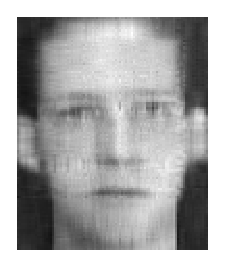
\includegraphics[scale=1.10]{img/singUV_noW_80.eps}}
  \subfigure[Con pesi centrati]
  {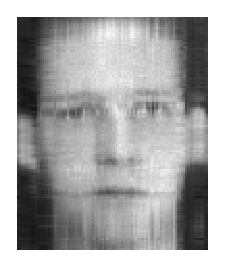
\includegraphics[scale=1.10]{img/singUV_80.eps}}
  \hspace{2mm}
  \subfigure[Originale]
  {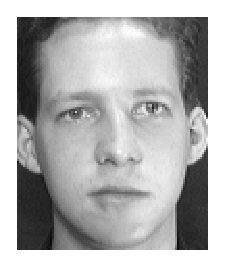
\includegraphics[scale=1.10]{img/original.eps}}
  \caption{Immagini dopo 80 iterazioni a confronto}
\end{figure}

\begin{figure}[h]
  \centering
  \subfigure[Senza pesi]
  {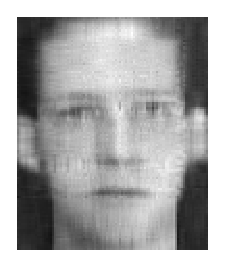
\includegraphics[trim = 5mm 20mm 5mm 12mm, clip=true, scale=1.60]{img/singUV_noW_80.eps}}
  \subfigure[Pesi centrati]
  {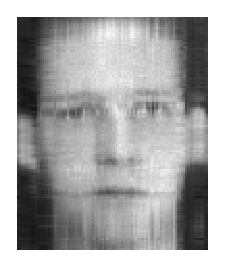
\includegraphics[trim = 5mm 20mm 5mm 12mm, clip=true, scale=1.60]{img/singUV_80.eps}}
  \subfigure[Originale]
  {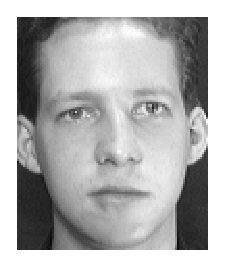
\includegraphics[trim = 5mm 20mm 5mm 12mm, clip=true, scale=1.60]{img/original.eps}}
  \caption{80 iterazioni, occhi a confronto}
\end{figure}

% \begin{figure}
%   \centering
%   \subfigure[Senza pesi]
%   {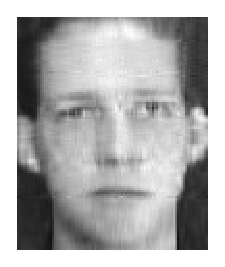
\includegraphics[scale=1.00]{img/singUV_noW_200.eps}}
%   \subfigure[Con pesi centrati]
%   {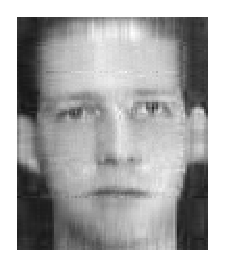
\includegraphics[scale=1.00]{img/singUV_200.eps}}
%   \hspace{2mm}
%   \subfigure[Originale]
%   {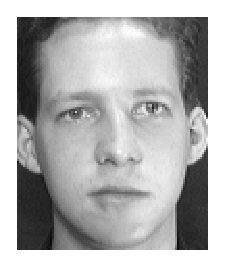
\includegraphics[scale=1.00]{img/original.eps}}
%   \caption{Immagini dopo 200 iterazioni a confronto}
% \end{figure}

\begin{figure}[h]
  \centering
  \subfigure[Senza pesi]
  {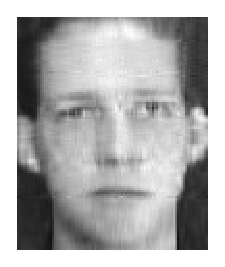
\includegraphics[trim = 5mm 20mm 5mm 12mm, clip=true, scale=1.70]{img/singUV_noW_200.eps}}
  \subfigure[Pesi centrati]
  {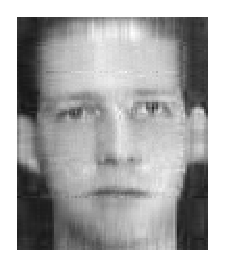
\includegraphics[trim = 5mm 20mm 5mm 12mm, clip=true, scale=1.70]{img/singUV_200.eps}}
  \subfigure[Originale]
  {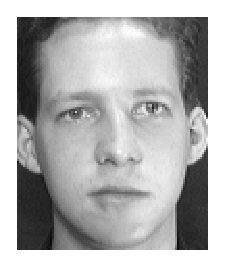
\includegraphics[trim = 5mm 20mm 5mm 12mm, clip=true, scale=1.70]{img/original.eps}}
  \caption{200 iterazioni, occhi a confronto}
\end{figure}

\begin{figure}[h]
  \centering
  Negativi a confronto:
  \subfigure
  {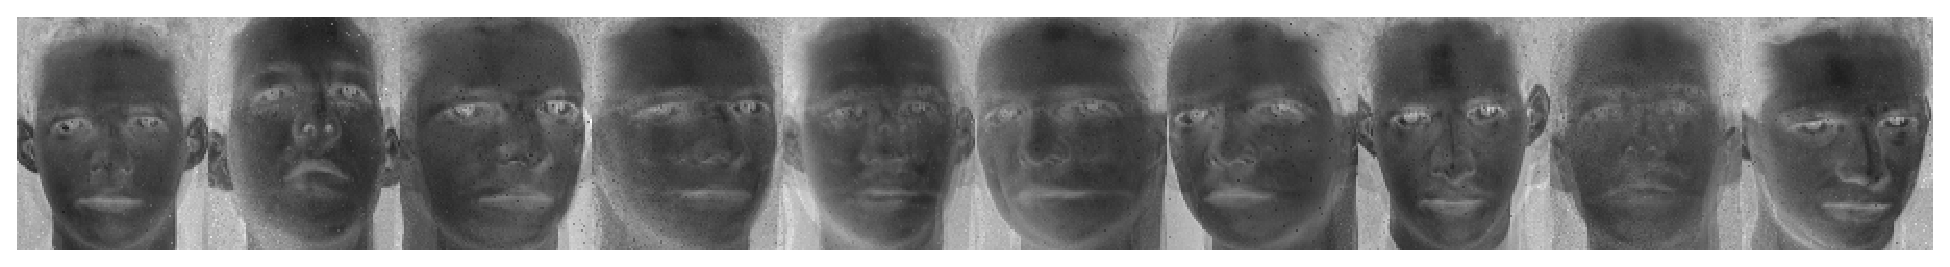
\includegraphics[scale=0.40]{img/negUV_noW.eps}}
  \subfigure
  {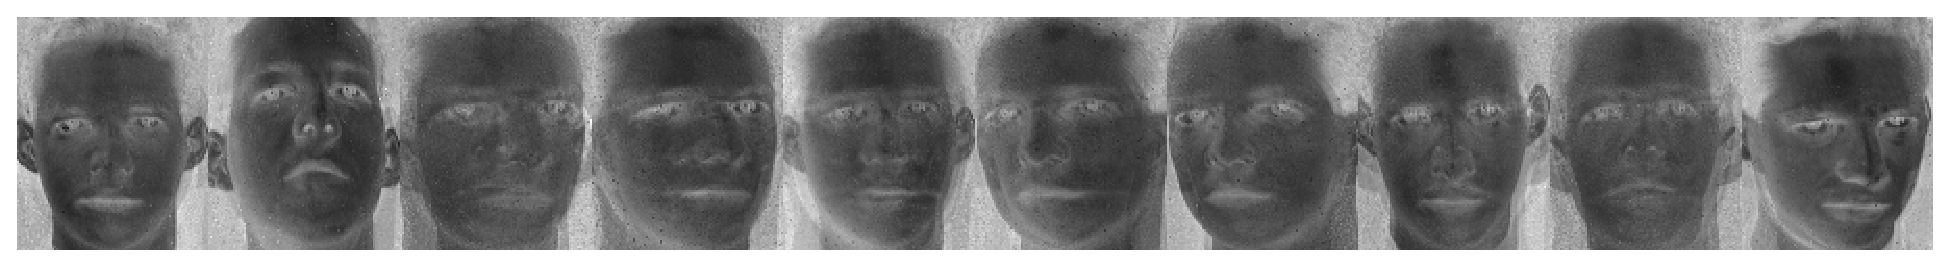
\includegraphics[scale=0.40]{img/negUV.eps}}
  % \vspace{2mm}
  \subfigure
  {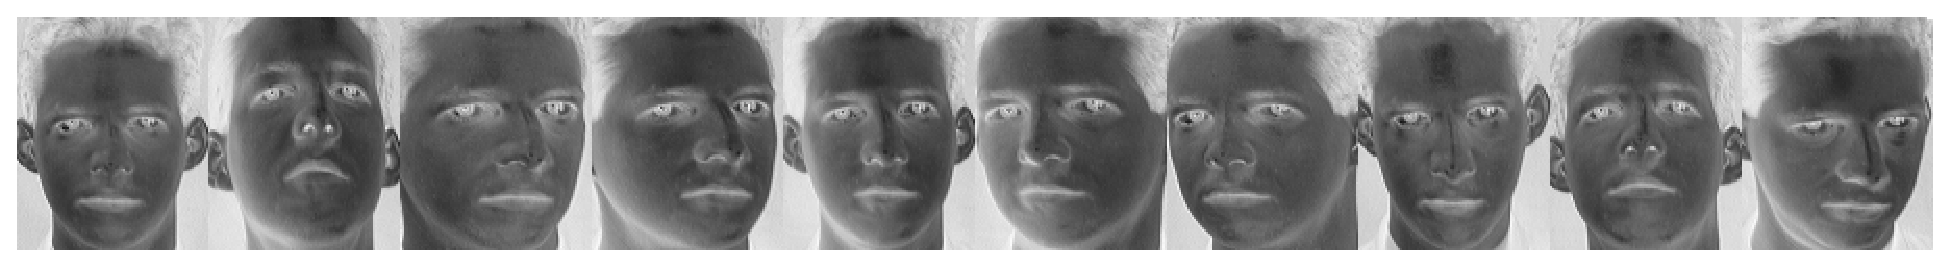
\includegraphics[scale=0.40]{img/negA.eps}}
  \caption{dall'alto: Negativi senza pesi, Negativi con pesi centrati, Originale}
\end{figure}

\clearpage{} % stampa pure quello che ti manca
%\nocite{*}
\begin{thebibliography}{}
\bibitem{wnmf}{%
    Vincent D. Blondel, Ngoc-Diep Ho, Paul van Dooren,
    \emph{Weighted Nonnegative Matrix Factorization
      and Face Feature Extraction},
    Universite\' catholique de Louvain, Belgium.
    Submitted to Image and Vision Computing, 
    March 2007
}\label{wnmf}

 \bibitem{orlfacedb}{%
     Olivetti Research Laboratory,
     \emph{\texttt{ORL} face database},
     Cambridge University Computer Laboratory,
     between April 1992 and April 1994, \verb-http://www.cl.cam.ac.uk/research/dtg/attarchive/facedatabase.html-
   }\label{ORL}

 \bibitem{pgma2pgmb}{%
     John Burkardt,
     \emph{\texttt{PGMA TO PGMB}},
     under GNU LGPL Licence,
     March 2011, \verb-http://people.sc.fsu.edu/~jburkardt/cpp_src/pgma_to_pgmb/pgma_to_pgmb.html-
   }\label{itm:A2B}

 \bibitem{pgmaio}{%
     John Burkardt,
     \emph{\texttt{PGMA IO}},
     under GNU LGPL Licence,
     December 2005, \verb-http://people.sc.fsu.edu/~jburkardt/f_src/pgma_io/pgma_io.html-
   }\label{itm:IO}

 \bibitem{leeseung}{%
     Daniel D. Lee and H. Sebastian Seung,
     \emph{Algorithms for Non-negative Matrix Factorization}
   }

 \bibitem{libnmf}{%
     A. Janecek, S. Schulze Grotthoff, W.N. Gansterer,
     \emph{\texttt{LIBNMF} – A LIBRARY FOR NONNEGATIVE MATRIX FACTORIZATION},
     University of Vienna, Austria,
     Faculty of Computer Science,
     Research Lab Computational Technologies \& Applications,
     from Computing and Informatics Volume 30, 2011
   }\label{libnmf}

\end{thebibliography}



\end{document}

